
% THIS IS AN EXAMPLE DOCUMENT FOR VLDB 2012
% based on ACM SIGPROC-SP.TEX VERSION 2.7
% Modified by  Gerald Weber <gerald@cs.auckland.ac.nz>
% Removed the requirement to include *bbl file in here. (AhmetSacan, Sep2012)
% Fixed the equation on page 3 to prevent line overflow. (AhmetSacan, Sep2012)

\documentclass{vldb}
\usepackage{graphicx}
\usepackage{balance}  % for  \balance command ON LAST PAGE  (only there!)

% ****************** sungsoo's packages ****************************************
\usepackage{times}
%                              My Commands
\newcommand{\bi}{\begin{itemize}}
\newcommand{\ei}{\end{itemize}}
\newcommand{\be}{\begin{enumerate}}
\newcommand{\ee}{\end{enumerate}}
\newcommand{\ii}{\item}
\newtheorem{Def}{Definition}
\newtheorem{Lem}{Lemma}
\usepackage{algorithm}
\usepackage{algorithmicx}
\usepackage{algpseudocode}

%\usepackage[]{algorithm2e}

\usepackage{graphicx}
\graphicspath{%
        {converted_graphics/}
        {./images/}
}
\usepackage{hyperref}
\usepackage{listings}
\usepackage{longtable}

% ****************** the following is needed for syntax highlighting
\usepackage{color}

\definecolor{dkgreen}{rgb}{0,0.6,0}
\definecolor{gray}{rgb}{0.5,0.5,0.5}
\definecolor{mauve}{rgb}{0.58,0,0.82}

\lstset{ %
  language=Java,                  % the language of the code
  basicstyle=\scriptsize,       % the size of the fonts that are used for the code
  numbers=left,                   % where to put the line-numbers
  numberstyle=\tiny\color{gray},  % the style that is used for the line-numbers
  stepnumber=1,                   % the step between two line-numbers. If it's 1, each line 
                                  % will be numbered
  numbersep=3.8pt,                  % how far the line-numbers are from the code
  backgroundcolor=\color{white},  % choose the background color. You must add \usepackage{color}
  showspaces=false,               % show spaces adding particular underscores
  showstringspaces=false,         % underline spaces within strings
  showtabs=false,                 % show tabs within strings adding particular underscores
  frame=false,                   % adds a frame around the code
  rulecolor=\color{black},        % if not set, the frame-color may be changed on line-breaks within not-black text (e.g. commens (green here))
  tabsize=2,                      % sets default tabsize to 2 spaces
  captionpos=b,                   % sets the caption-position to bottom
  breaklines=true,                % sets automatic line breaking
  breakatwhitespace=false,        % sets if automatic breaks should only happen at whitespace
  title=\lstname,                 % show the filename of files included with \lstinputlisting;
                                  % also try caption instead of title
  keywordstyle=\color{blue},          % keyword style
  commentstyle=\color{dkgreen},       % comment style
  stringstyle=\color{mauve},         % string literal style
  escapeinside={\%*}{*)},            % if you want to add a comment within your code
  morekeywords={*,...}               % if you want to add more keywords to the set
}
% ****************** end of sungsoo's packages ****************************************


\begin{document}

% ****************** TITLE ****************************************

%\title{A Sample {\ttlit Proceedings of the VLDB Endowment} Paper in LaTeX
%Format\titlenote{for use with vldb.cls}}

\title{Introduction to the Data Warehouse}

% possible, but not really needed or used for PVLDB:
%\subtitle{[Extended Abstract]
%\titlenote{A full version of this paper is available as\textit{Author's Guide to Preparing ACM SIG Proceedings Using \LaTeX$2_\epsilon$\ and BibTeX} at \texttt{www.acm.org/eaddress.htm}}}

% ****************** AUTHORS **************************************

% You need the command \numberofauthors to handle the 'placement
% and alignment' of the authors beneath the title.
%
% For aesthetic reasons, we recommend 'three authors at a time'
% i.e. three 'name/affiliation blocks' be placed beneath the title.
%
% NOTE: You are NOT restricted in how many 'rows' of
% "name/affiliations" may appear. We just ask that you restrict
% the number of 'columns' to three.
%
% Because of the available 'opening page real-estate'
% we ask you to refrain from putting more than six authors
% (two rows with three columns) beneath the article title.
% More than six makes the first-page appear very cluttered indeed.
%
% Use the \alignauthor commands to handle the names
% and affiliations for an 'aesthetic maximum' of six authors.
% Add names, affiliations, addresses for
% the seventh etc. author(s) as the argument for the
% \additionalauthors command.
% These 'additional authors' will be output/set for you
% without further effort on your part as the last section in
% the body of your article BEFORE References or any Appendices.

\numberofauthors{1} %  in this sample file, there are a *total*
% of EIGHT authors. SIX appear on the 'first-page' (for formatting
% reasons) and the remaining two appear in the \additionalauthors section.

\author{
% You can go ahead and credit any number of authors here,
% e.g. one 'row of three' or two rows (consisting of one row of three
% and a second row of one, two or three).
%
% The command \alignauthor (no curly braces needed) should
% precede each author name, affiliation/snail-mail address and
% e-mail address. Additionally, tag each line of
% affiliation/address with \affaddr, and tag the
% e-mail address with \email.
%
% 1st. author
\alignauthor
Sung-Soo Kim\\ %\titlenote{Dr.~Trovato insisted his name be first.}\\
       \affaddr{Data Management Research Section}\\
       \affaddr{Electronics and Telecommunications Research Institute}\\
       \affaddr{128 Gajeong-ro, Yuseong-gu}\\
       \affaddr{Daejeon, South Korea}\\
       \email{\normalsize \it sungsoo@etri.re.kr}
% 2nd. author
%\alignauthor
%G.K.M. Tobin\titlenote{The secretary disavows
%any knowledge of this author's actions.}\\
%       \affaddr{Institute for Clarity in Documentation}\\
%       \affaddr{P.O. Box 1212}\\
%       \affaddr{Dublin, Ohio 43017-6221}\\
%       \email{webmaster@marysville-ohio.com}
% 3rd. author
%\alignauthor Lars Th{\Large{\sf{\o}}}rv{$\ddot{\mbox{a}}$}ld\titlenote{This author is the
%one who did all the really hard work.}\\
%       \affaddr{The Th{\large{\sf{\o}}}rv{$\ddot{\mbox{a}}$}ld Group}\\
%       \affaddr{1 Th{\large{\sf{\o}}}rv{$\ddot{\mbox{a}}$}ld Circle}\\
%       \affaddr{Hekla, Iceland}\\
%       \email{larst@affiliation.org}
%\and  % use '\and' if you need 'another row' of author names
% 4th. author
%\alignauthor Lawrence P. Leipuner\\
%       \affaddr{Brookhaven Laboratories}\\
%       \affaddr{Brookhaven National Lab}\\
%       \affaddr{P.O. Box 5000}\\
%       \email{lleipuner@researchlabs.org}
% 5th. author
%\alignauthor Sean Fogarty\\
%       \affaddr{NASA Ames Research Center}\\
%       \affaddr{Moffett Field}\\
%       \affaddr{California 94035}\\
%       \email{fogartys@amesres.org}
% 6th. author
%\alignauthor Charles Palmer\\
%       \affaddr{Palmer Research Laboratories}\\
%       \affaddr{8600 Datapoint Drive}\\
%       \affaddr{San Antonio, Texas 78229}\\
%       \email{cpalmer@prl.com}
}
% There's nothing stopping you putting the seventh, eighth, etc.
% author on the opening page (as the 'third row') but we ask,
% for aesthetic reasons that you place these 'additional authors'
% in the \additional authors block, viz.
%\additionalauthors{Additional authors: John Smith (The Th{\o}rv\"{a}ld Group, {\texttt{jsmith@affiliation.org}}), Julius P.~Kumquat
%(The \raggedright{Kumquat} Consortium, {\small \texttt{jpkumquat@consortium.net}}), and Ahmet Sacan (Drexel University, {\small \texttt{ahmetdevel@gmail.com}})}
%\date{30 July 1999}
% Just remember to make sure that the TOTAL number of authors
% is the number that will appear on the first page PLUS the
% number that will appear in the \additionalauthors section.


\maketitle

\begin{abstract}
This technical report explores the main concepts and components of business intelligence and
decision support systems that gather, generate, and present information for business
decision makers, focusing especially on the use of \textit{data warehouses}.
Data are crucial raw material in this information age, and data storage and management have
become the focus of database design and implementation.
The data warehouse extracts or obtains its
data from operational databases as well as from external sources, providing a more
comprehensive data pool.
\end{abstract}

\section{Introduction}

%\begin{figure}[htb]
%\centering
%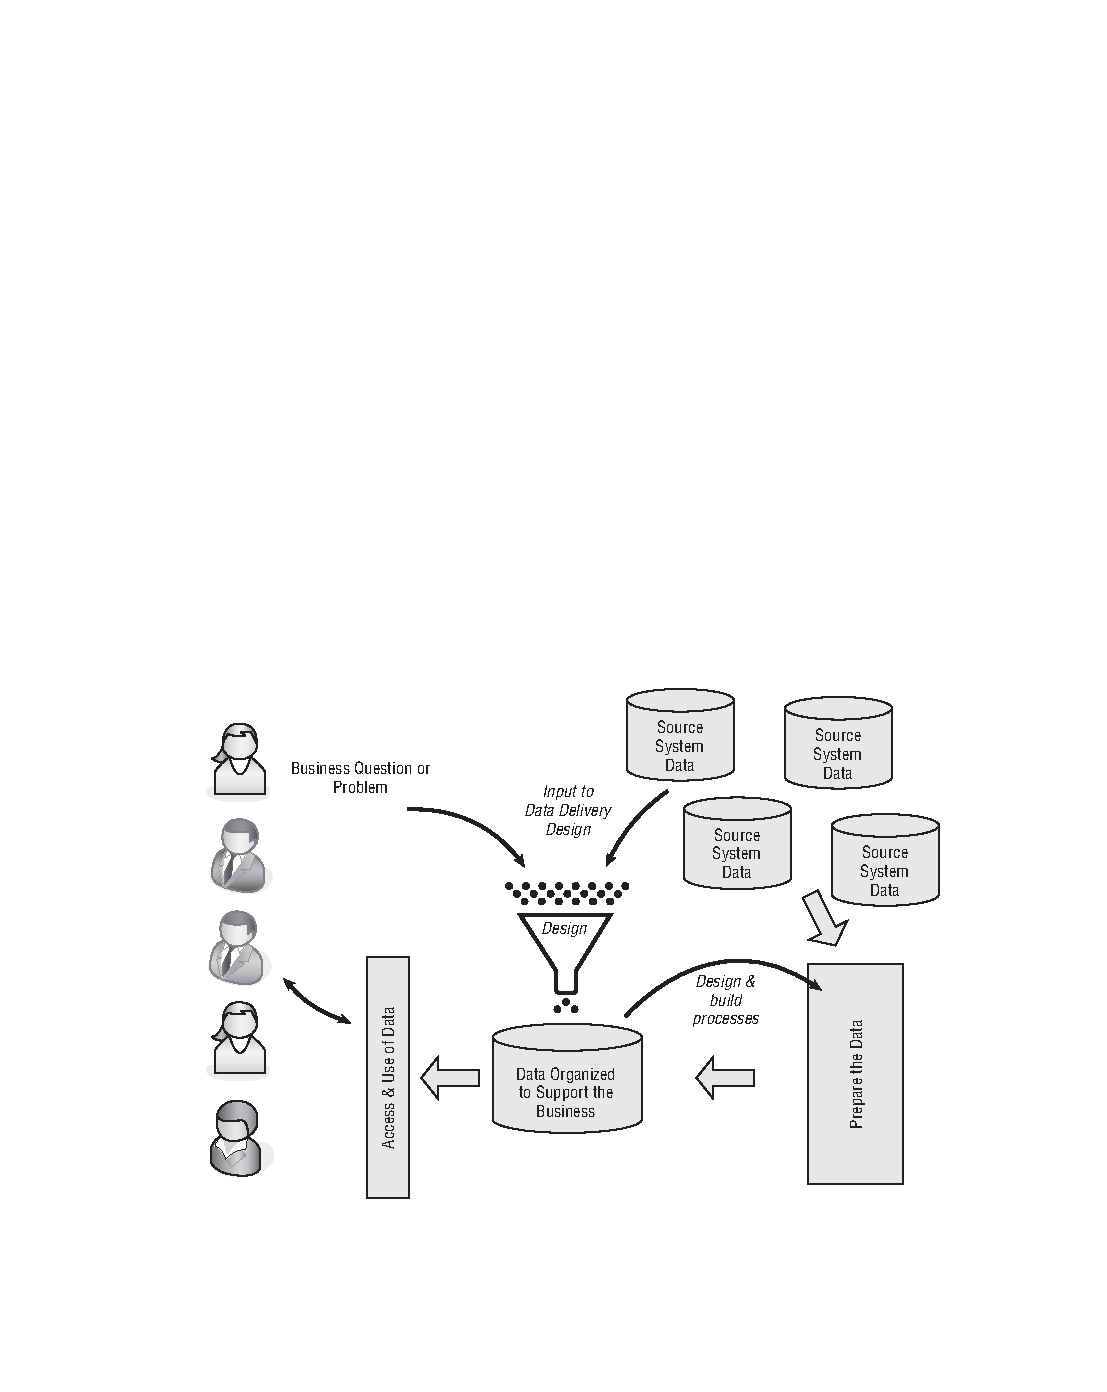
\includegraphics[width=0.48\textwidth]{datawarehouse}
%\caption{Optimal data warehouse design and development sequence}
%\label{fig:datawarehouse}
%\end{figure}

Organizations tend to grow and prosper as they gain a better understanding of their environment. Most managers want
to be able to track daily transactions to evaluate how the business is performing. By tapping into the operational
database, management can develop strategies to meet organizational goals. In addition, data analysis can provide
information about short-term tactical evaluations and strategies such as these: Are our sales promotions working? What
market percentage are we controlling? Are we attracting new customers? Tactical and strategic decisions are also
shaped by constant pressure from external and internal forces, including globalization, the cultural and legal
environment, and (perhaps most importantly) technology.

Given the many and varied competitive pressures, managers are always looking for a competitive advantage through
product development and maintenance, service, market positioning, sales promotion, and so on. Managers understand
that the business climate is dynamic, and thus, mandates their prompt reaction to change in order to remain
competitive. In addition, the modern business climate requires managers to approach increasingly complex problems
that involve a rapidly growing number of internal and external variables. It should also come as no surprise that interest
is growing in creating support systems dedicated to facilitating quick decision making in a complex environment.

Different managerial levels require different decision support needs. For example, transaction-processing systems,
based on operational databases, are tailored to serve the information needs of people who deal with short-term
inventory, accounts payable, and purchasing. Middle-level managers, general managers, vice presidents, and presidents
focus on strategic and tactical decision making. Those managers require detailed information designed to help
them make decisions in a complex data and analysis environment.

Companies and software vendors addressed these multilevel decision support needs by creating independent
applications to fit the needs of particular areas (finance, customer management, human resources, product support,
etc.). Applications were also tailored to different industry sectors such as education, retail, health care, or financial. This
approach worked well for some time, but changes in the business world (globalization, expanding markets, mergers
and acquisitions, increased regulation, and more) called for new ways of integrating and managing data across levels,
sectors, and geographic locations. This more comprehensive and integrated decision support framework within
organizations became known as business intelligence \cite{carloDB:2011}.

\section{The Data Warehouse}
Large companies have presences in many places, each of which may generate
a large volume of data. For instance, large retail chains have hundreds or thousands
of stores, whereas insurance companies may have data from thousands
of local branches. Further, large organizations have a complex internal organization
structure, and therefore different data may be present in different locations,
or on different operational systems, or under different schemas. For instance,
manufacturing-problem data and customer-complaint data may be stored on different
database systems. Organizations often purchase data fromexternal sources,
such as mailing lists that are used for product promotions, or credit scores of customers
that are provided by credit bureaus, to decide on credit-worthiness of
customers.

Corporate decision makers require access to information from multiple such
sources. Setting up queries on individual sources is both cumbersome and inefficient.
Moreover, the sources of datamay store only current data,whereas decision
makers may need access to past data as well; for instance, information about how
purchase patterns have changed in the past year could be of great importance.
Data warehouses provide a solution to these problems.

A \textit{data warehouse} is a repository (or archive) of information gathered from
multiple sources, stored under a unified schema, at a single site \cite{Silberschatz:2010}. Once gathered,
the data are stored for a long time, permitting access to historical data. Thus,
data warehouses provide the user a single consolidated interface to data, making
decision-support queries easier to write. Moreover, by accessing information
for decision support from a data warehouse, the decision maker ensures that
online transaction-processing systems are not affected by the decision-support
workload.

\begin{figure*}[htb]
\centering
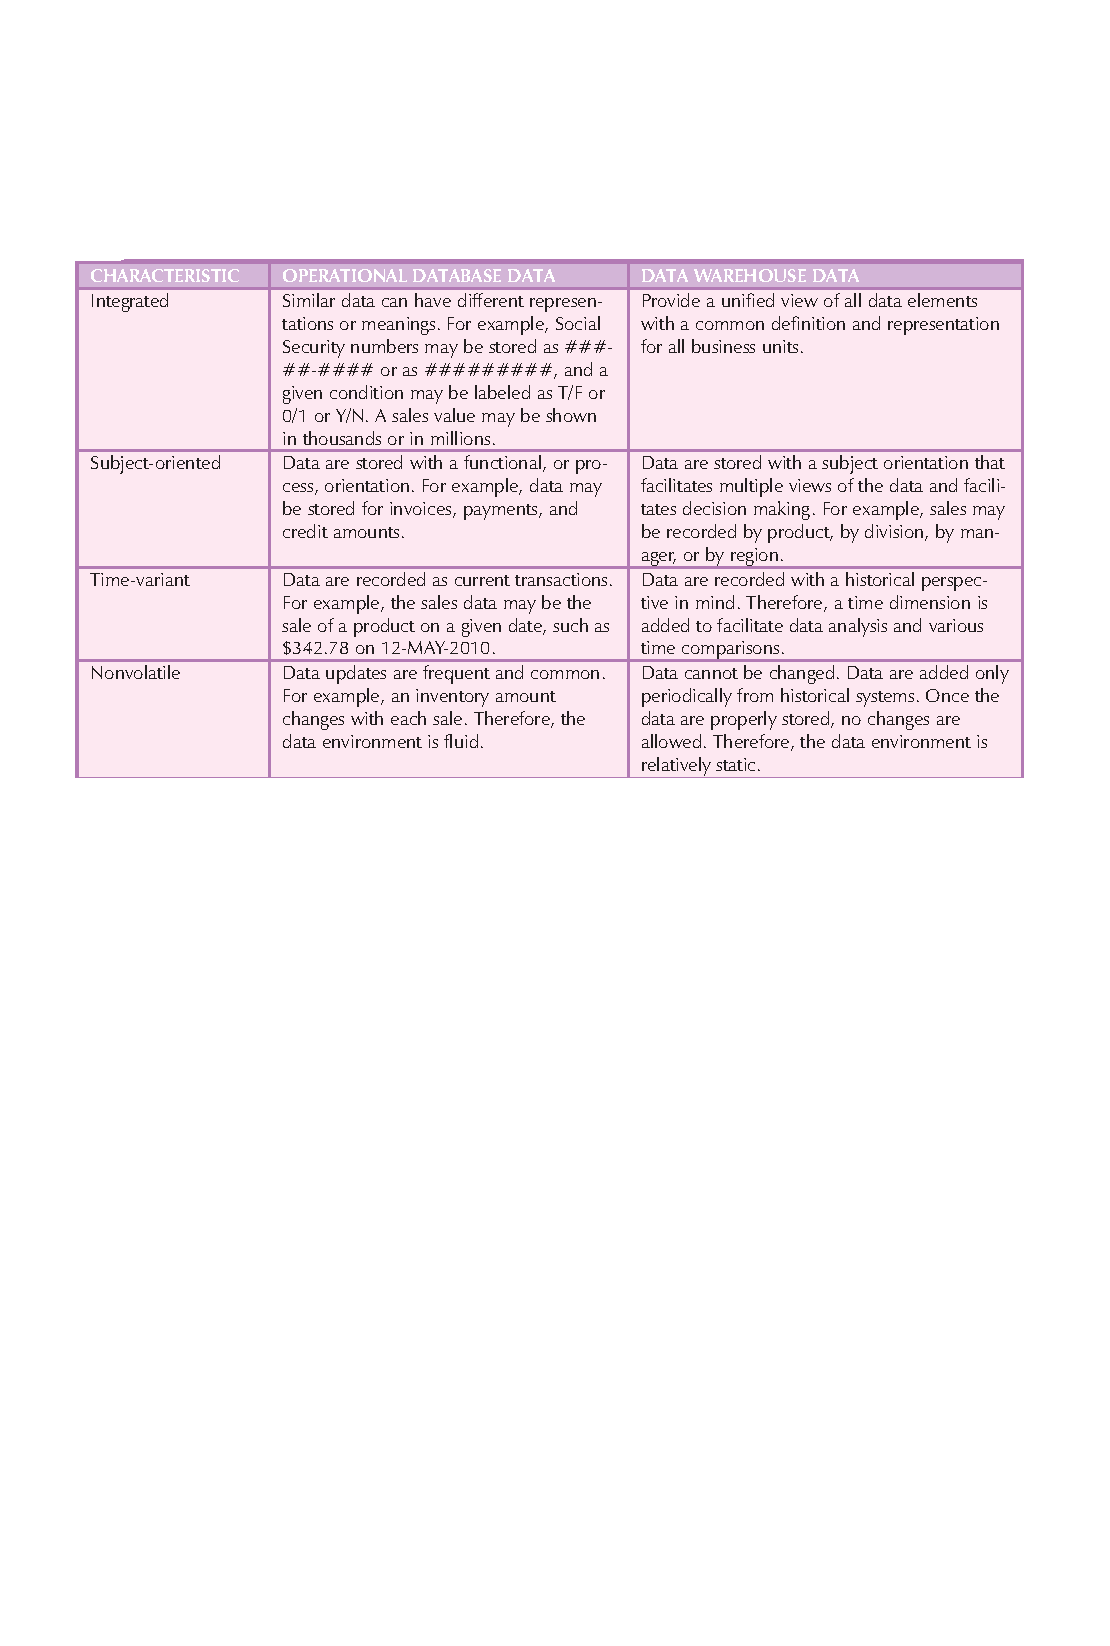
\includegraphics[width=0.8\textwidth]{data-comparison}
\caption{Characteristics of Data Warehouse Data and Operational Database Data}
\label{fig:data-comparison}
\end{figure*}

Bill Inmon, the acknowledged “father” of the data warehouse, defines the term as “an integrated, subject-oriented,
time-variant, nonvolatile collection of data (italics added for emphasis) that provides support for decision making.”

To understand that definition, let’s take a more detailed look at its components.

\bi
\ii \textbf{Integrated.} The data warehouse is a centralized, consolidated database that integrates data derived from the
entire organization and from multiple sources with diverse formats. Data integration implies that all business
entities, data elements, data characteristics, and business metrics are described in the same way throughout
the enterprise. Although this requirement sounds logical, you would be amazed to discover how many different
measurements for “sales performance” can exist within an organization; the same scenario holds true for any
other business element. For instance, the status of an order might be indicated with text labels such as “open,”
“received,” “canceled,” and “closed” in one department and as “1,” “2,” “3,” and “4” in another department.
A student’s status might be defined as “freshman,” “sophomore,” “junior,” or “senior” in the accounting
department and as “FR,” “SO,” “JR,” or “SR” in the computer information systems department. To avoid the
potential format tangle, the data in the data warehouse must conform to a common format acceptable
throughout the organization. This integration can be time-consuming, but once accomplished, it enhances
decision making and helps managers better understand the company’s operations. This understanding can be
translated into recognition of strategic business opportunities.

\ii \textbf{Subject-oriented.} Data warehouse data are arranged and optimized to provide answers to questions coming
from diverse functional areas within a company. Data warehouse data are organized and summarized by topic,
such as sales, marketing, finance, distribution, and transportation. For each topic, the data warehouse contains
specific subjects of interest—products, customers, departments, regions, promotions, and so on. This form of
data organization is quite different from the more functional or process-oriented organization of typical
transaction systems. For example, an invoicing system designer concentrates on designing normalized data
structures (relational tables) to support the business process by storing invoice components in two tables:
INVOICE and INVLINE. In contrast, the data warehouse has a subject orientation. Data warehouse designers
focus specifically on the data rather than on the processes that modify the data. (After all, data warehouse data
are not subject to numerous real-time data updates!) Therefore, instead of storing an invoice, the data
warehouse stores its “sales by product” and “sales by customer” components because decision support
activities require the retrieval of sales summaries by product or customer.

\ii  \textbf{Time-variant.} In contrast to operational data, which focus on current transactions, warehouse data represent the
flow of data through time. The data warehouse can even contain projected data generated through statistical and
other models. It is also time-variant in the sense that once data are periodically uploaded to the data warehouse,
all time-dependent aggregations are recomputed. For example, when data for previous weekly sales are uploaded
to the data warehouse, the weekly, monthly, yearly, and other time-dependent aggregates for products,
customers, stores, and other variables are also updated. Because data in a data warehouse constitute a snapshot
of the company history as measured by its variables, the time component is crucial. The data warehouse contains
a time ID that is used to generate summaries and aggregations by week, month, quarter, year, and so on. Once
the data enter the data warehouse, the time ID assigned to the data cannot be changed.

\ii \textbf{Nonvolatile.} Once data enter the data warehouse, they are never removed. Because the data in the warehouse
represent the company’s history, the operational data, representing the near-term history, are always added to
it. Because data are never deleted and new data are continually added, the data warehouse is always growing.
That’s why the DBMS must be able to support multigigabyte and even multiterabyte or greater databases,
operating on multiprocessor hardware. Figure \ref{fig:data-comparison} summarizes the differences between data warehouses and
operational databases.
\ei

In summary, the data warehouse is usually a read-only database optimized for data analysis and query processing.
Typically, data are extracted from various sources and are then transformed and integrated—in other words, passed
through a data filter—before being loaded into the data warehouse. As mentioned, this process of extracting,
transforming, and loading the aggregated data into the data warehouse is known as ETL. Figure \ref{fig:etl-process} illustrates the ETL process to create a data warehouse from operational data.

\begin{figure}[htb]
\centering
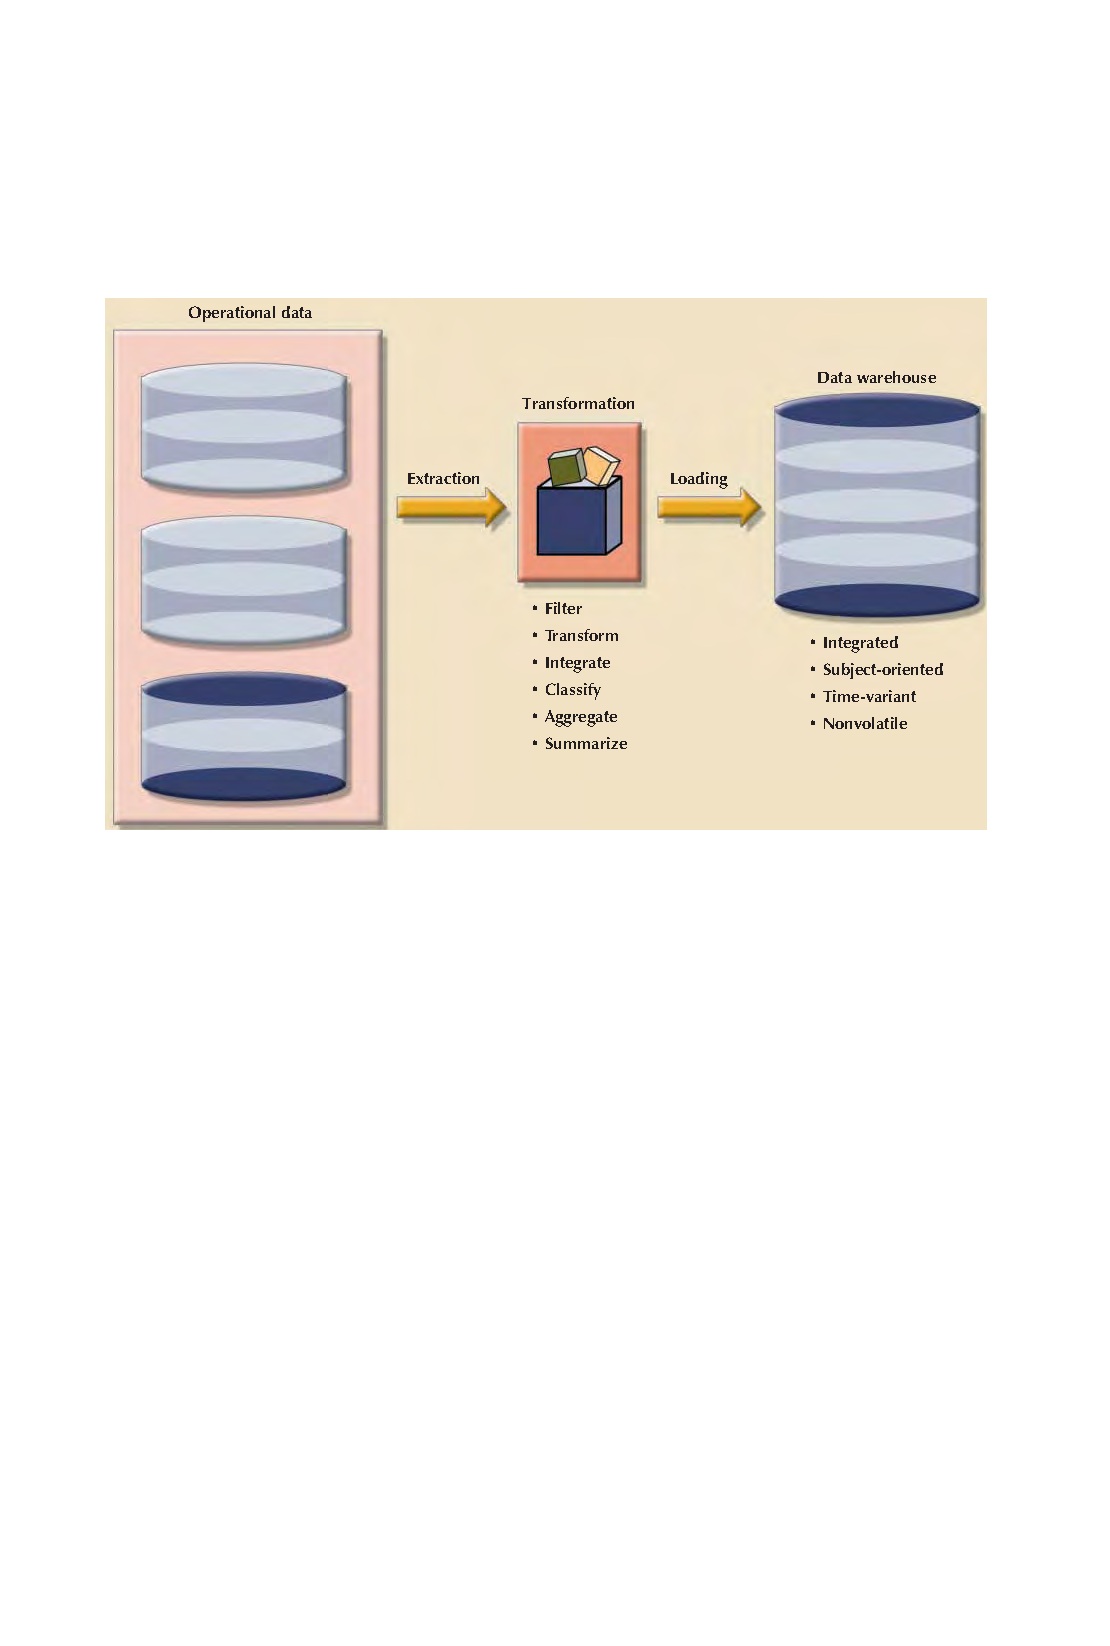
\includegraphics[width=0.48\textwidth]{etl-process}
\caption{The ETL Process}
\label{fig:etl-process}
\end{figure}

Although the centralized and integrated data warehouse can be a very attractive proposition that yields many benefits,
managers may be reluctant to embrace this strategy. Creating a data warehouse requires time, money, and
considerable managerial effort. Therefore, it is not surprising that many companies begin their foray into data
warehousing by focusing on more manageable data sets that are targeted to meet the special needs of small groups
within the organization. These smaller data stores are called data marts. A \textit{data mart} is a small, single-subject data
warehouse subset that provides decision support to a small group of people. In addition, a data mart could also be
created from data extracted from a larger data warehouse with the specific function to support faster data access to
a target group or function. That is, data marts and data warehouses can coexist within a business intelligence
environment.

Some organizations choose to implement data marts not only because of the lower cost and shorter implementation
time but also because of the current technological advances and inevitable “people issues” that make data marts
attractive. Powerful computers can provide a customized decision support system to small groups in ways that might
not be possible with a centralized system. Also, a company’s culture may predispose its employees to resist major
changes, but they might quickly embrace relatively minor changes that lead to demonstrably improved decision
support. In addition, people at different organizational levels are likely to require data with different summarization,
aggregation, and presentation formats. Data marts can serve as a test vehicle for companies exploring the potential
benefits of data warehouses. By gradually migrating from data marts to data warehouses, a specific department’s
decision support needs can be addressed within a reasonable time frame (six months to one year) as opposed to the
longer time frame usually required to implement a data warehouse (one to three years). Information technology (IT)
departments also benefit from this approach because their personnel have the opportunity to learn the issues and
develop the skills required to create a data warehouse.

The only difference between a data mart and a data warehouse is the size and scope of the problem being solved.
Therefore, the problem definitions and data requirements are essentially the same for both. To be useful, the data
warehouse must conform to uniform structures and formats to avoid data conflicts and to support decision making. 
In fact, before a decision support database can be considered a true data warehouse, it must conform to the rules
described in the next section.

\section{Components of Data Warehouse}
Figure \ref{fig:architecture} shows the architecture of a typical data warehouse, and illustrates the
gathering of data, the storage of data, and the querying and data analysis support.

\begin{figure}[htb]
\centering
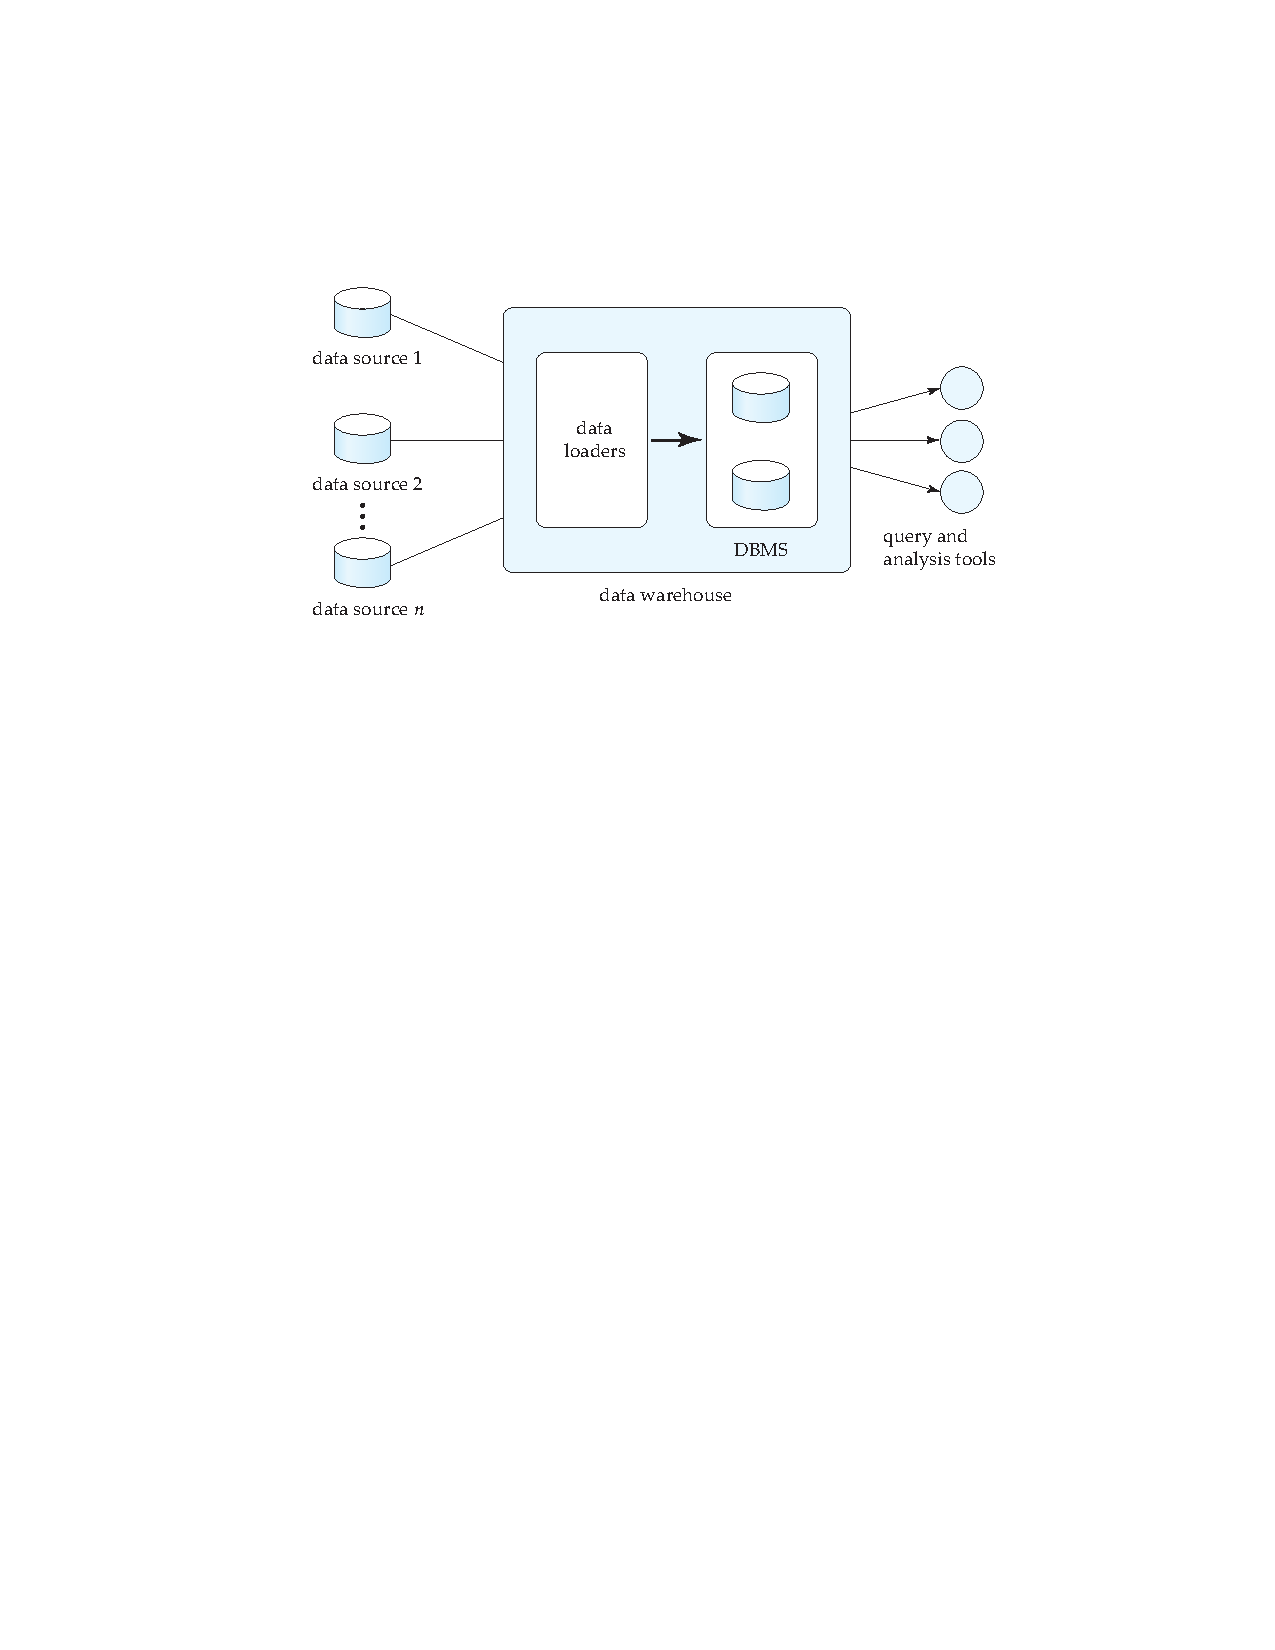
\includegraphics[width=0.48\textwidth]{architecture}
\caption{Data-Warehouse Architecture}
\label{fig:architecture}
\end{figure}

Among the issues to be addressed in building a warehouse are the following:

\bi
\ii \textbf{When and how to gather data.} In a \textit{source-driven architecture} for gathering
data, the data sources transmit new information, either continually (as
transaction processing takes place), or periodically (nightly, for example).
In a \textit{destination-driven architecture}, the datawarehouse periodically sends
requests for new data to the sources.

Unless updates at the sources are replicated at the warehouse via twophase
commit, thewarehousewill never be quite up-to-datewith the sources.
Two-phase commit is usually far too expensive to be an option, so data
warehouses typically have slightly out-of-date data. That, however, is usually
not a problem for decision-support systems.

\ii \textbf{What schema to use.} Data sources that have been constructed independently
are likely to have different schemas. In fact, they may even use different data
models. Part of the task of a warehouse is to perform schema integration,
and to convert data to the integrated schema before they are stored. As a
result, the data stored in the warehouse are not just a copy of the data at the
sources. Instead, they can be thought of as a materialized view of the data at
the sources.

\ii \textbf{Data transformation and cleansing.} The task of correcting and preprocessing
data is called \textit{data cleansing}. Data sources often deliver data with numerous
minor inconsistencies, which can be corrected. For example, names are often
misspelled, and addressesmay have street, area, or city namesmisspelled, or
postal codes entered incorrectly. These can be corrected to a reasonable extent
by consulting a database of street names and postal codes in each city. The
approximate matching of data required for this task is referred to as \textit{fuzzy
lookup}.

Address lists collected from multiple sources may have duplicates that
need to be eliminated in a \textit{merge–purge operation} (this operation is also
referred to as \textit{deduplication}). 
Records for multiple individuals in a house may be grouped together so only one mailing is sent to each house; this operation is called \textit{householding}.

Data may be \textit{transformed} in ways other than cleansing, such as changing
the units of measure, or converting the data to a different schema by joining
data from multiple source relations. Data warehouses typically have graphical
tools to support data transformation. Such tools allow transformation to
be specified as boxes, and edges can be created between boxes to indicate the
flow of data. Conditional boxes can route data to an appropriate next step in
transformation. 

\ii \textbf{How to propagate updates.} Updates on relations at the data sources must
be propagated to the data warehouse. If the relations at the data warehouse
are exactly the same as those at the data source, the propagation is straightforward.
If they are not, the problem of propagating updates is basically the
\textit{view-maintenance} problem.

\ii \textbf{What data to summarize.} The raw data generated by a transaction-processing
system may be too large to store online. However, we can answer many
queries by maintaining just summary data obtained by aggregation on a
relation, rather than maintaining the entire relation. For example, instead of
storing data about every sale of clothing, we can store total sales of clothing
by item name and category.

Suppose that a relation r has been replaced by a summary relation s.
Users may still be permitted to pose queries as though the relation r were
available online. If the query requires only summary data, it may be possible
to transform it into an equivalent one using s instead.
\ei

The different steps involved in getting data into a data warehouse are called
\textit{extract}, \textit{transform}, and \textit{load} or ETL tasks as shown in Figure \ref{fig:etl-process}; extraction refers to getting data from
the sources, while load refers to loading the data into the data warehouse.

\subsection{Data Warehouse Manager}
The data warehouse manager’s role represents the driving force behind the data warehouse environment from the IT organization. This individual is often given direct responsibility for the funds for the data warehouse project. This is the primary visionary for data warehousing in the organization, and the lead systems professional who is responsible for building and sustaining the data warehouse. The data warehouse manager continues to have responsibility for the data warehouse after a project is complete and oversees support, maintenance, and growth.

Data warehousing focuses on the management of five primary data flows, namely the \textit{inflow}, \textit{upflow}, \textit{downflow}, \textit{outflow}, and \textit{metaflow}  \cite{Thomas:DW}. The data flows within a data warehouse are shown in Figure \ref{fig:dwflow}. The processes associated with each data flow include:

\begin{figure}[htb]
\centering
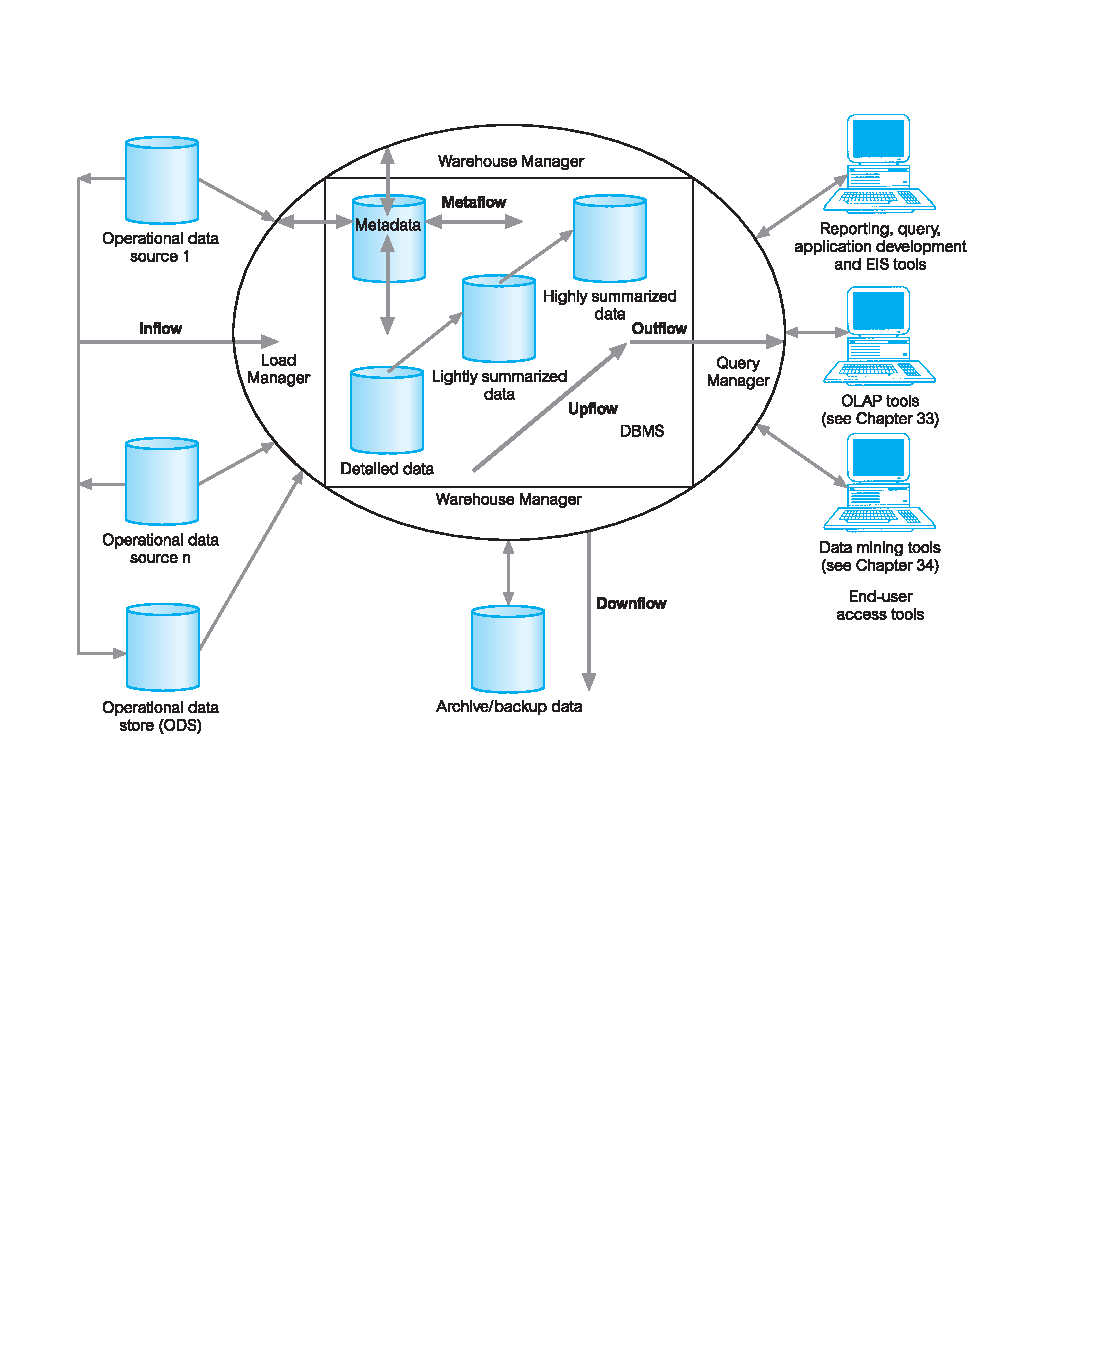
\includegraphics[width=0.48\textwidth]{dwflow}
\caption{Information flows of a data warehouse}
\label{fig:dwflow}
\end{figure}

\bi
\ii \textbf{Inflow} Extraction, cleansing, and loading of the source data.
\ii \textbf{Upflow} Adding value to the data in the warehouse through summarizing, packaging,  and distribution of the data.
\ii \textbf{Downflow} Archiving and backing-up the data in the warehouse.
\ii \textbf{Outflow} Making the data available to end-users.
\ii \textbf{Metaflow} Managing the metadata.
\ei

The data warehouse manager must set the overall direction of the data warehouse. This is done in conjunction with key business management. This includes making sure that a sound technical and data architecture is developed. The data warehouse manager is the focal point for blending industry best practices with internal best practices to develop an overall methodology and techniques that will ensure the long-term success of data warehousing within the organization. This includes adapting \textit{system development life cycle} (SDLC) practices and the definition of standard deliverables to meet the unique data warehousing needs.

If there are many data warehousing projects underway, the data warehouse manager would then be involved in coordinating and leveraging resources across the projects. These resources could include \textit{people} as well as \textit{technology} .

\section{Twelve Rules} % That Define A Data Warehouse}
In 1994, William H. Inmon and Chuck Kelley created 12 rules defining a data warehouse, which summarize many of
the points made in this chapter about data warehouses.
\be
\ii The data warehouse and operational environments are \textit{separated}.
\ii The data warehouse data are \textit{integrated}.
\ii The data warehouse contains \textit{historical} data over a long time.
\ii The data warehouse data are \textit{snapshot} data captured at a given point in time.
\ii The data warehouse data are \textit{subject oriented}.
\ii The data warehouse data are \textit{mainly read-only} with \textit{periodic batch updates} from operational data. \textit{No online updates} are allowed.
\ii The data warehouse development life cycle differs from classical systems development. The data warehouse development is \textit{data-driven}; the classical approach is \textit{process-driven}.
\ii The data warehouse contains data with several \textit{levels of detail}: current detail data, old detail data, lightly
summarized data, and highly summarized data.
\ii The data warehouse environment is characterized by \textit{read-only transactions} to very large data sets. The
operational environment is characterized by numerous update transactions to a few data entities at a time.
\ii The data warehouse environment has a system that traces data sources, transformations, and storage.
\ii The data warehouse’s \textit{metadata} are a critical component of this environment. The metadata identify and define
all data elements. The metadata provide the source, transformation, integration, storage, usage, relationships,
and history of each data element.
\ii The data warehouse contains a \textit{chargeback mechanism} for resource usage that enforces optimal use of the data
by end users.
\ee

Note how those 12 rules capture the complete data warehouse life cycle—from its introduction as an entity separate
from the operational data store to its components, functionality, and management processes. The next section
illustrates the historical progression of decision support architectural styles. This discussion will help you understand
how the data store components evolved to produce the data warehouse.

\section{Warehouse Schemas}
Data warehouses typically have schemas that are designed for data analysis, using
tools such as OLAP tools. Thus, the data are usually \textit{multidimensional} data, with
dimension attributes and measure attributes. Tables containing multidimensional
data are called \textbf{fact tables} and are usually very large. A table recording \textit{sales}
information for a retail store, with one tuple for each item that is sold, is a typical
example of a fact table. The dimensions of the sales table would include what the
item is (usually an item identifier such as that used in bar codes), the date when
the item is sold, which location (store) the item was sold from, which customer
bought the item, and so on. The measure attributes may include the number of
items sold and the price of the items.

To minimize storage requirements, dimension attributes are usually short
identifiers that are foreign keys into other tables called \textbf{dimension tables}. For
instance, a fact table \textit{sales} would have attributes \textit{item\_id}, \textit{store\_id}, \textit{customer\_id}, and
\textit{date}, and measure attributes \textit{number} and \textit{price}. The attribute store id is a foreign
key into a dimension table store, which has other attributes such as store location
(city, state, country). The \textit{item\_id} attribute of the \textit{sales} table would be a foreign key
into a dimension table \textit{item\_info}, which would contain information such as the
name of the item, the category to which the item belongs, and other item details
such as color and size. The \textit{customer\_id} attribute would be a foreign key into a
\textit{customer} table containing attributes such as name and address of the customer.
We can also view the \textit{date} attribute as a foreign key into a \textit{date\_info} table giving the
month, quarter, and year of each date.

\begin{figure}[htb]
\centering
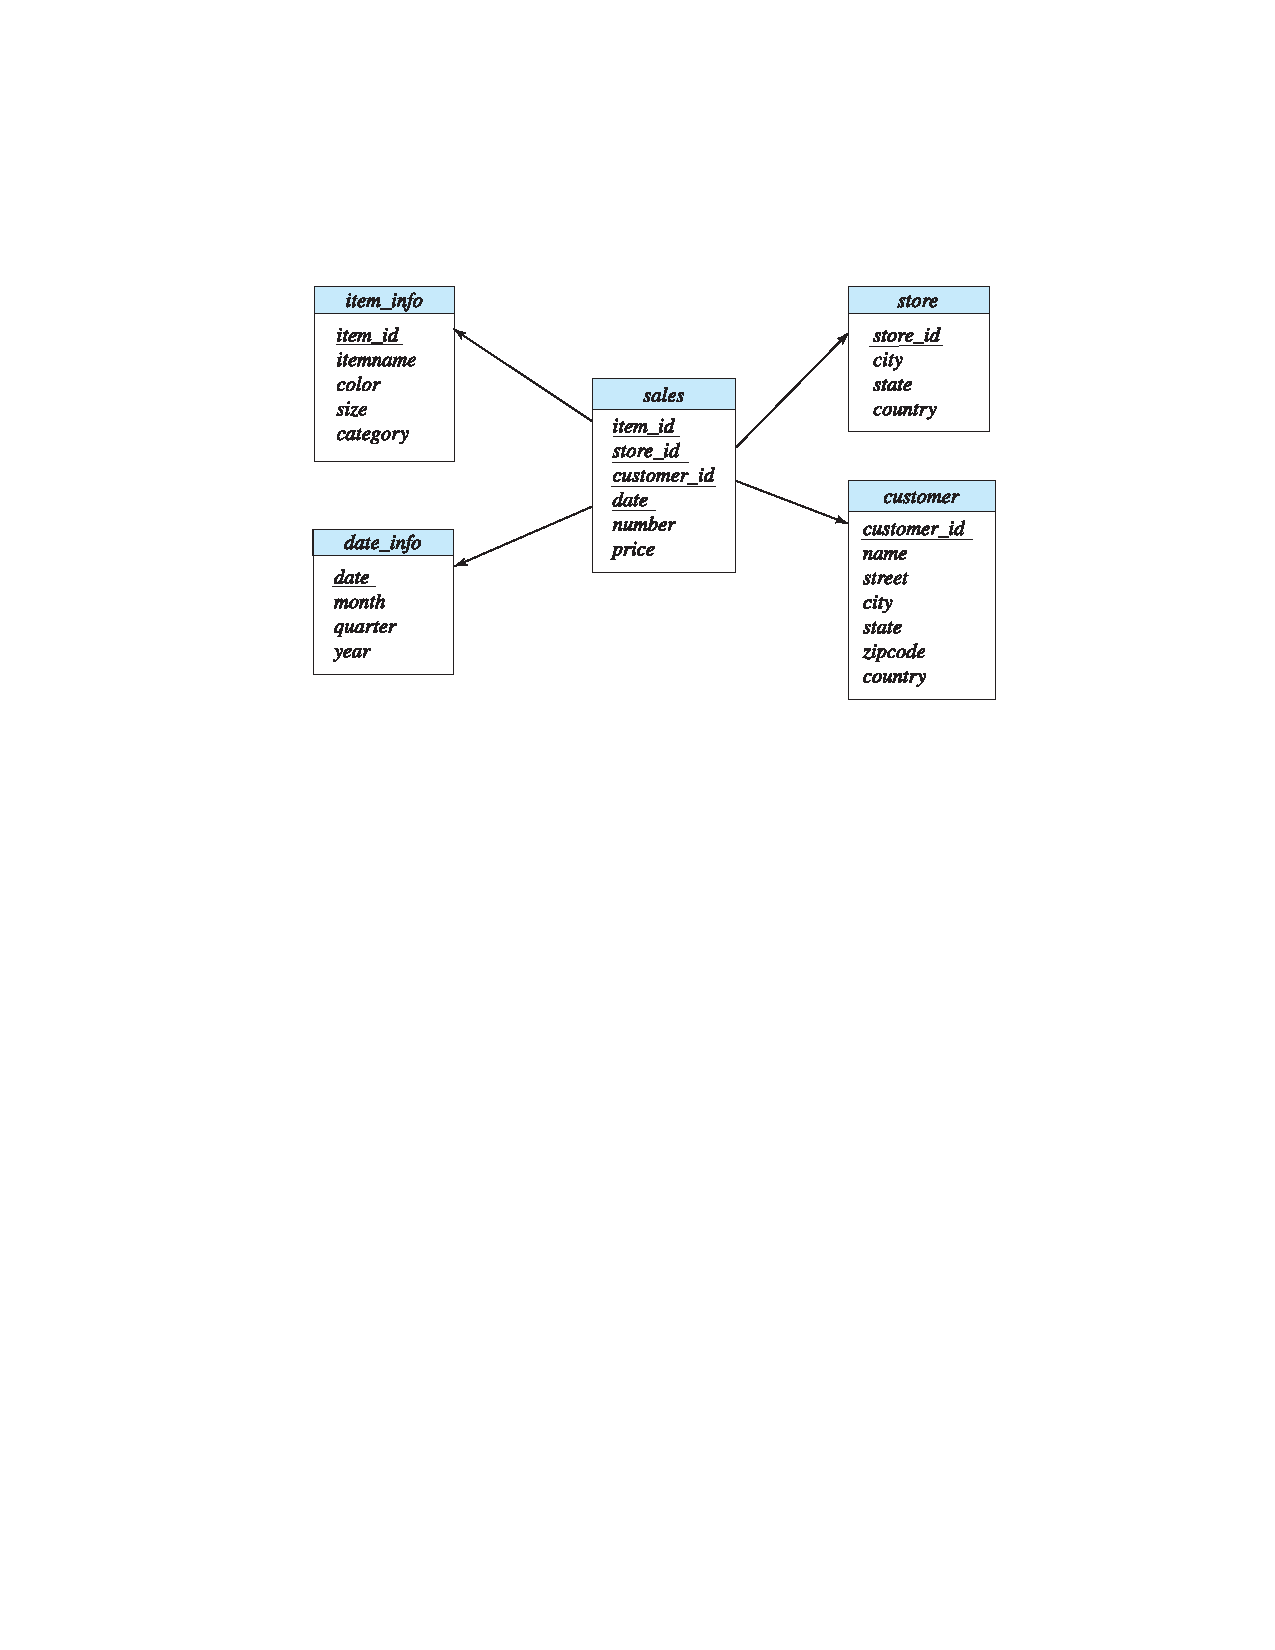
\includegraphics[width=0.48\textwidth]{starschema}
\caption{Star Schema for a Data Warehouse}
\label{fig:starschema}
\end{figure}

The resultant schema appears in Figure \ref{fig:starschema}. Such a schema, with a fact table,
multiple dimension tables, and foreign keys from the fact table to the dimension
tables, is called a \textbf{star schema}. More complex data-warehouse designs may have
multiple levels of dimension tables; for instance, the \textit{item\_info} table may have an
attribute \textit{manufacturer\_id} that is a foreign key into another table giving details of
the manufacturer. Such schemas are called \textbf{snowflake schemas}. Complex datawarehouse
designs may also have more than one fact table.

\section{Summary}
In this technical report, we have reviewed the main concepts of the data warehouse.
Businesses have begun to exploit the burgeoning data online to make better
decisions about their activities, such as what items to stock and how best to target
customers to increase sales. 

There are two aspects to exploiting such data. The first aspect is to gather data from multiple sources into a central repository, called a \textit{data warehouse}. Issues involved in warehousing include techniques for dealing
with dirty data, that is, data with some errors, and with techniques for efficient
storage and indexing of large volumes of data.
Data warehouses help gather and archive important operational data.Warehouses
are used for decision support and analysis on historical data, for
instance, to predict trends. Data cleansing from input data sources is often a
major task in data warehousing.Warehouse schemas tend to be multidimensional,
involving one or a few very large fact tables and several much smaller
dimension tables.

The second aspect is to analyze the gathered data to find information or
knowledge that can be the basis for business decisions. Some kinds of data analysis
can be done by using SQL constructs for online analytical processing (OLAP).

Building a data warehouse is challenging, but it can also provide great rewards.
This technical report offered a general overview of data warehousing and illustrated how it can serve as a potential foundation for realizing business value. 


\bibliographystyle{abbrv}
\bibliography{sqlonhadoop}

\end{document}
